\begin{figure}[t]
  \centering
  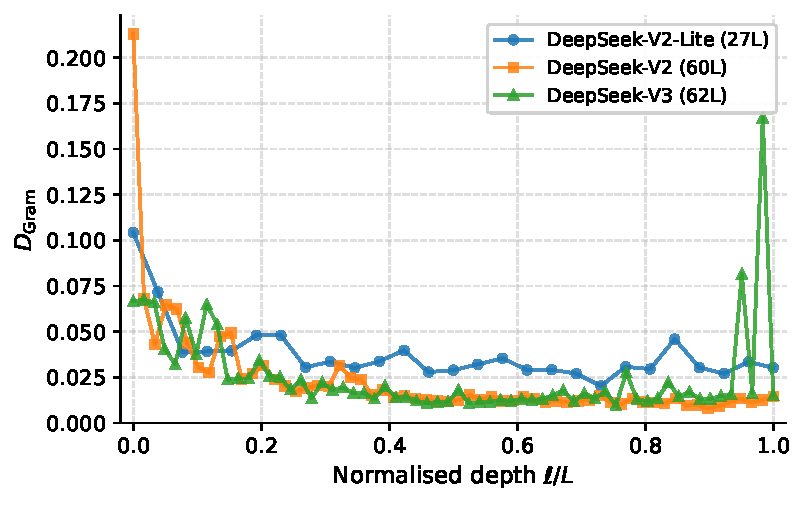
\includegraphics[width=\columnwidth]{fig_ushape}
  \caption{%
    Gram distance $D_{\text{Gram}}$ between the effective key and value
    operators $\widetilde{W}_K$ and $\widetilde{W}_V$ as a function of
    normalised depth $\ell/L$, measured on DeepSeek-V2-Lite ($L{=}27$),
    DeepSeek-V2 ($L{=}60$), and DeepSeek-V3 ($L{=}62$).
    All three networks share the same qualitative profile: large geometric
    divergence in the first few layers, rapid convergence to a low-alignment
    plateau through the middle of the network, and a pronounced late-layer
    spike (most visible in V3) before the final representations are formed.
    This U-shaped pattern holds across a ${\sim}40{\times}$ range of model
    scale, suggesting it is a structural property of the MLA
    parameterisation rather than an artefact of a particular model size.
    Full per-layer numerical values are listed in
    Appendix~\ref{app:per-layer-tables}.%
  }
  \label{fig:ushape}
\end{figure}
